% Testbed diagram. Built from infra/docker-compose.yml (service wiring), experiments/fault_injector.py
% (one Toxiproxy proxy per service) and each service's application.yml (the ten breakers).
% Designed for two-column width (~7 in); all text is \footnotesize (8 pt at 10 pt base).
\documentclass[tikz,border=2pt]{standalone}
\usetikzlibrary{arrows.meta}
\tikzset{
  svc/.style={draw, rounded corners=1pt, minimum width=1.9cm, minimum height=0.8cm,
              font=\footnotesize, align=center},
  edge/.style={-{Stealth[length=4pt]}, line width=0.6pt},
  fan/.style={edge, dashed},
  hot/.style={edge, line width=1.8pt},
  tp/.style={draw, fill=black, minimum size=0.2cm, inner sep=0pt},
  cb/.style={font=\footnotesize, align=center, inner sep=1pt, fill=white},
}
\begin{document}
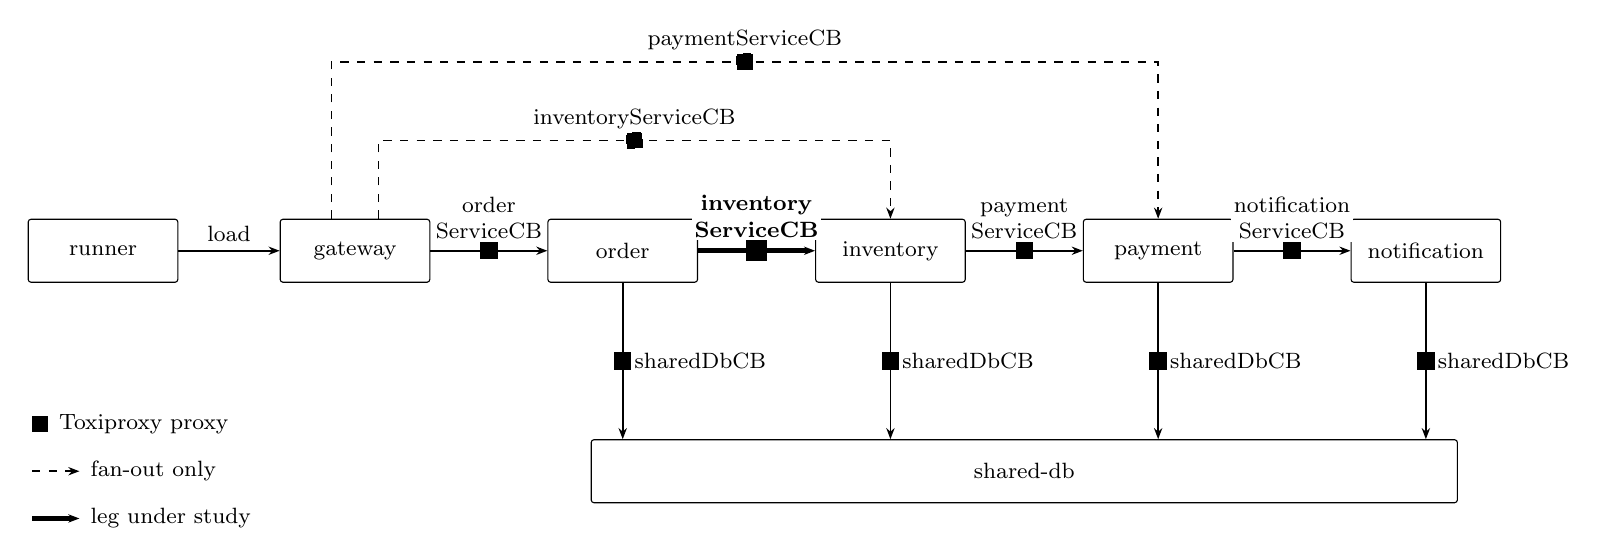
\begin{tikzpicture}
  % services, left to right
  \node[svc] (run) at (0,0)    {runner};
  \node[svc] (gw)  at (3.2,0)  {gateway};
  \node[svc] (ord) at (6.6,0)  {order};
  \node[svc] (inv) at (10.0,0) {inventory};
  \node[svc] (pay) at (13.4,0) {payment};
  \node[svc] (not) at (16.8,0) {notification};
  \node[svc, minimum width=11cm] (sdb) at (11.7,-2.8) {shared-db};

  % entry: runner drives load into the gateway directly (no proxy)
  \draw[edge] (run.east) -- node[cb, above=2pt] {load} (gw.west);

  % linear chain, each edge through a Toxiproxy proxy; order$\to$inventory highlighted
  \draw[edge] (gw.east)  -- node[tp] {} node[cb, above=3pt] {order\\ServiceCB} (ord.west);
  \draw[hot]  (ord.east) -- node[tp] {} node[cb, above=3pt] {\textbf{inventory}\\\textbf{ServiceCB}} (inv.west);
  \draw[edge] (inv.east) -- node[tp] {} node[cb, above=3pt] {payment\\ServiceCB} (pay.west);
  \draw[edge] (pay.east) -- node[tp] {} node[cb, above=3pt] {notification\\ServiceCB} (not.west);

  % fan-out only: gateway also calls inventory and payment directly (dashed)
  \draw[fan] ([xshift=0.3cm]gw.north) -- ([xshift=0.3cm]gw.north |- 0,1.4)
             -- node[tp] {} node[cb, above=3pt] {inventoryServiceCB} (inv.north |- 0,1.4)
             -- (inv.north);
  \draw[fan] ([xshift=-0.3cm]gw.north) -- ([xshift=-0.3cm]gw.north |- 0,2.4)
             -- node[tp] {} node[cb, above=3pt] {paymentServiceCB} (pay.north |- 0,2.4)
             -- (pay.north);

  % every service reaches shared-db through its proxy and its own sharedDbCB
  \foreach \s in {ord, inv, pay, not} {
    \draw[edge] (\s.south) -- node[tp] {} node[cb, right=3pt] {sharedDbCB} (\s.south |- sdb.north);
  }

  % legend
  \node[tp] at (-0.8,-2.2) {};
  \node[cb, anchor=west] at (-0.6,-2.2) {Toxiproxy proxy};
  \draw[fan] (-0.9,-2.8) -- (-0.3,-2.8);
  \node[cb, anchor=west] at (-0.2,-2.8) {fan-out only};
  \draw[hot] (-0.9,-3.4) -- (-0.3,-3.4);
  \node[cb, anchor=west] at (-0.2,-3.4) {leg under study};
\end{tikzpicture}
\end{document}
